\documentclass[class=report, crop=false, 12pt,a4paper]{standalone}
\usepackage{enumitem}
\usepackage{multicol}
\usepackage{graphicx}
\usepackage{float}
\usepackage{amsmath}
\usepackage{amssymb}
\usepackage{mathtools}
\usepackage{siunitx}
\usepackage{commath}
\usepackage{array}
\usepackage{natbib}
\usepackage[a4paper,width=150mm,top=25mm,bottom=25mm]{geometry}
\setlength{\parindent}{0pt}
\begin{document}
\begin{center}
    09/10/2020
\end{center}
\section{Actions and Deformations}
\subsection{Vector Quantities}
A vector is a quantity defined by \textbf{magnitude} and \textbf{direction}. Mechanical actions (forces and moments) can be represented as \textbf{vectors}. \\\\
Vector quantities can be decomposed in components, that can be conveniently oriented with the Cartesian reference system.
\begin{figure}[H]
  \centering
  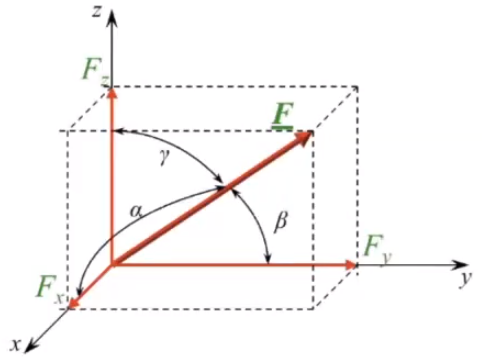
\includegraphics[width = 0.5 \textwidth]{../img/vectordecomposition.PNG}
\end{figure}
\begin{gather}
  F_x = F \cdot \cos \alpha \ \ \ \ \ \ \ \ \ \ M_x = M \cdot \cos \alpha \\
  F_y = F \cdot \cos \beta \ \ \ \ \ \ \ \ \ \ M_y = M \cdot \cos \beta \\
  F_z = F \cdot \cos \gamma \ \ \ \ \ \ \ \ \ \ M_z = M \cdot \cos \gamma
\end{gather}
On the other hand, a set of vector forces can be composed in a resultant force applied to any point P, and the moment they produce about P. 
\begin{figure}[H]
  \centering
  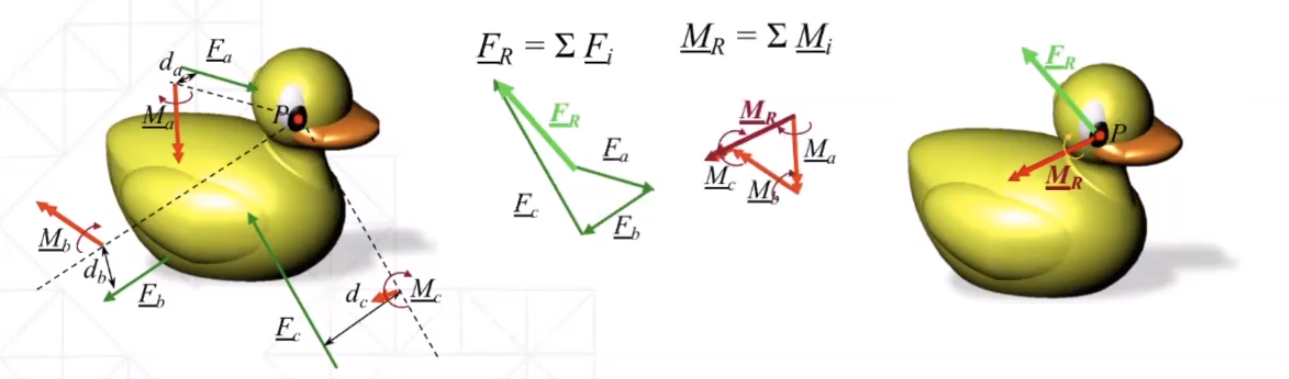
\includegraphics[width = 1 \textwidth]{../img/forcesandmoments.PNG}
\end{figure}
\begin{gather}
  \vec{F_R} = \sum \vec{F_i} \ \ \ \ \ \ \ \ \ \ \vec{M_R} = \sum \vec{F_i} \\
  F_R = \sqrt{(F_x)^2 + (F_y)^2 + (F_z)^2} \\
  M_R = \sqrt{(M_x)^2 + (M_y)^2 + (M_z)^2}
\end{gather}
\subsection{Equilibrium State}
If a configuration is in equilibrium, the resultant of all external forces and moments is zero. This can be expressed mathematically in the following 6 equations:
\begin{center}
  \begin{tabular}{ c c c } 
   $\sum F_x = 0$ & \ $\sum F_y = 0$ & \ $\sum F_z = 0$ \\
   $\sum M_x = 0$ & \ $\sum M_y = 0$ & \ $\sum M_z = 0$
  \end{tabular}
\end{center}
These equations have to be valid for the entire body, and for any of its portions.
\subsection{Deformations}
Mechanical actions produce \textbf{deformations} in the body. These can be:
\begin{itemize}[noitemsep]
  \item Tension
  \item Compression
  \item Bending
  \item Twisting
\end{itemize}
These deformations translate into local strains and are opposed and balanced by internal reaction forces (and stresses), that guarantee the structural congruence of the body.
\begin{figure}[H]
  \centering
  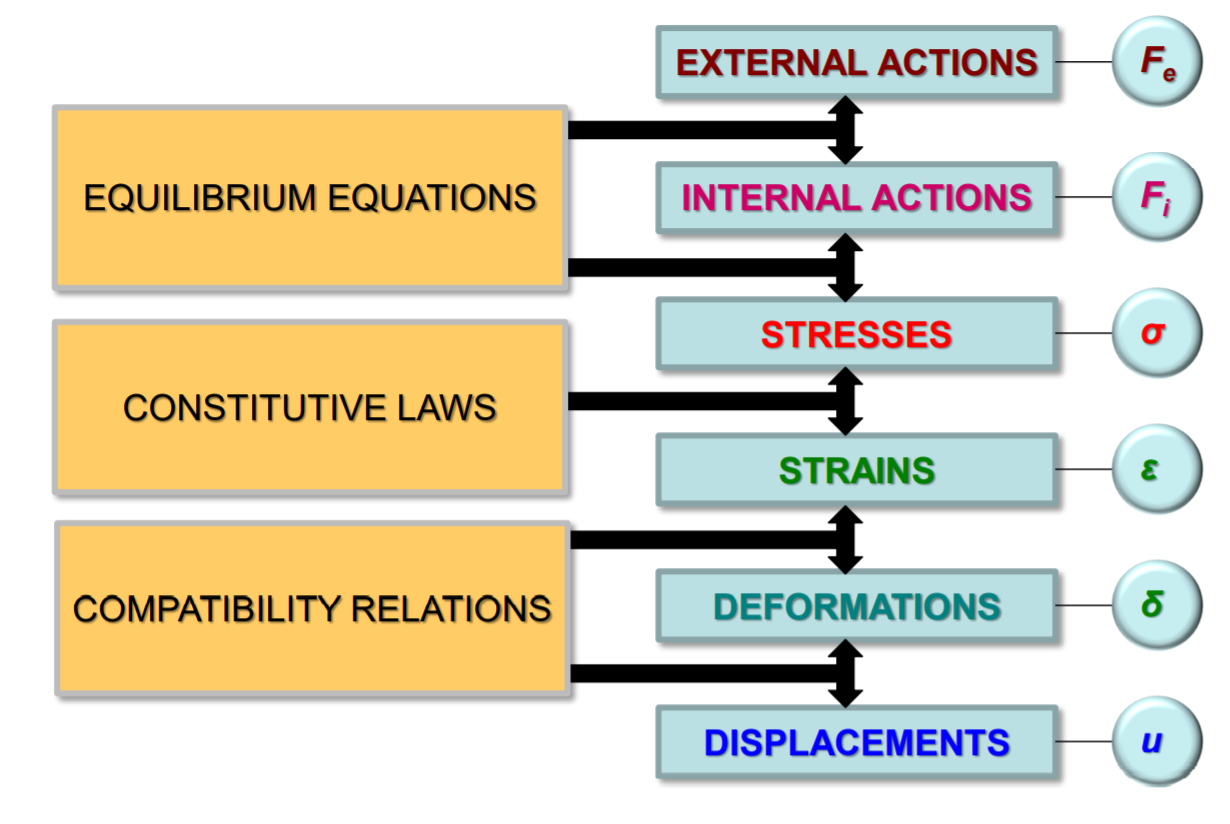
\includegraphics[width = 0.6 \textwidth]{../img/solidmechanicsequation.PNG}
  \caption{Solid Mechanics Equation: When dealing with mechanical action problems, the actions listed in the flowchart above occur, starting with external/internal forces and ending with displacements/deformations}
\end{figure}
\section{Degree of Freedom and Supports}
We define \textbf{degree of freedom} of a system as all the basic kinematical parameters (or all the forms of movement) allowed. A rigid body in the space, in a coordinate system, has 6 degrees of freedom: \\\\
3 translations along the coordinate axes $x$, $y$ and $z$
\begin{figure}[H]
  \centering
  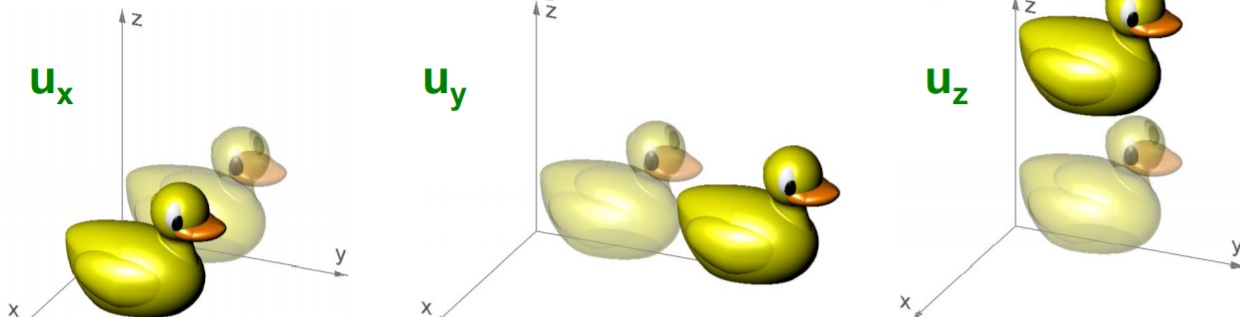
\includegraphics[width = 0.9 \textwidth]{../img/axistranslations.PNG}
\end{figure}
3 rotations about the coordinate axes $x$, $y$ and $z$
\begin{figure}[H]
  \centering
  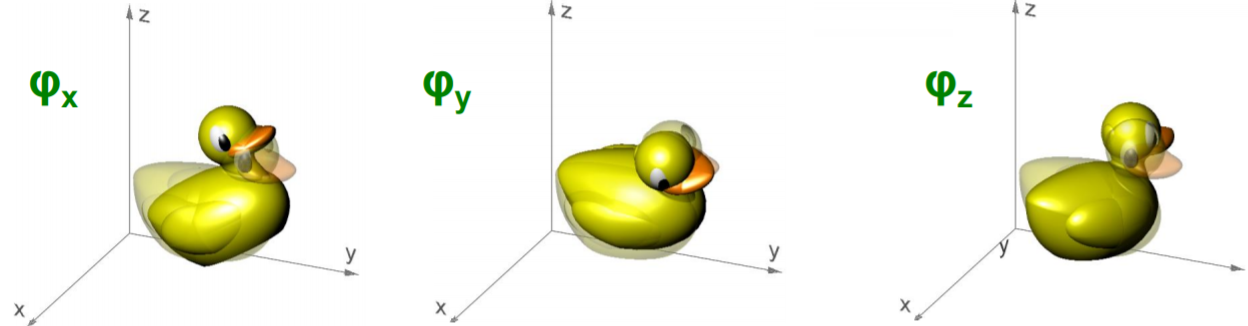
\includegraphics[width = 0.9 \textwidth]{../img/axisrotations.PNG}
\end{figure}
The total translational and rotational movement of an object can be shown with the following expression:
\begin{center}
  $\vec{u} = \left[ \begin{array}{cccccc} u_x \\ u_y \\ u_z \\ \phi_x \\ \phi_y \\ \phi_z \end{array}\right]$
\end{center}
In a 2D plane, the degree of freedom reduces to pnly 3 variables:
\begin{center}
  $\vec{u} = \left[ \begin{array}{ccc} u_x \\ u_y \\ \phi_z \end{array}\right]$
\end{center}
\subsection{Constraint}
We define \textbf{constraint} as a limitation of the degree of freedom of the system. The most common constraints are:
\begin{itemize}[noitemsep]
  \item Supports providing the required reacting forces to maintain overall equilibrium
  \item Connections providing reaction forces between two components of the system
\end{itemize}
The table below summarizes the different types of supports (constraints) that will be used throughout the course:
\begin{center}
  \begin{tabular}{ |c|c|c|c| } 
   \hline
   Fixed & Rotating & Roller & Sliding \\
   \hline
   
\includegraphics[width = 0.2 \textwidth]{../img/fixedsupport.PNG} & 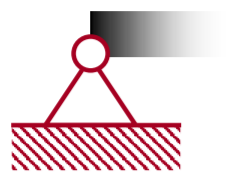
\includegraphics[width = 0.2 \textwidth]{../img/rotatingsupport.PNG} & 
\includegraphics[width = 0.2 \textwidth]{../img/rollersupport.PNG} & 
\includegraphics[width = 0.2 \textwidth]{../img/slidingsupport.PNG} \\
   \hline
   $\vec{u} = \left[ \begin{array}{ccc} 0 \\ 0 \\ 0 \end{array}\right]$ & $\vec{u} = \left[ \begin{array}{ccc} 0 \\ 0 \\ \phi \end{array}\right]$ & $\vec{u} = \left[ \begin{array}{ccc} u_x \\ 0 \\ \phi \end{array}\right]$ & $\vec{u} = \left[ \begin{array}{ccc} u_x \\ 0 \\ 0 \end{array}\right]$ \\
   \hline
   $\vec{R} = \left[ \begin{array}{ccc} R_x \\ R_y \\ M_z \end{array}\right]$ & $\vec{R} = \left[ \begin{array}{ccc} R_x \\ R_y \\ 0 \end{array}\right]$ & $\vec{R} = \left[ \begin{array}{ccc} 0 \\ R_y \\ 0 \end{array}\right]$ & $\vec{R} = \left[ \begin{array}{ccc} 0 \\ R_y \\ M \end{array}\right]$ \\
   \hline
  \end{tabular}
\end{center}
\section{Beams and Sign Conventions}
Structures are sets of solid bodies components with the function of carrying loads. All solid bodies are 3-dimensional, however, often it is possible to identify some dimension that is more relevant. Many structures can be analysed as bi-dimensional (2D) or mono-dimensional (1D).
\subsection{Types of Structures}
\subsubsection{Bi-dimensional Structures}
If one of the dimensions is negligible compared to the other two, the
structure can be studied as bi-dimensional. Some examples are:
\begin{itemize}[noitemsep]
  \item Plates
  \item Membranes
  \item Shells (Only locally 2D)
\end{itemize}
\begin{figure}[H]
  \centering
  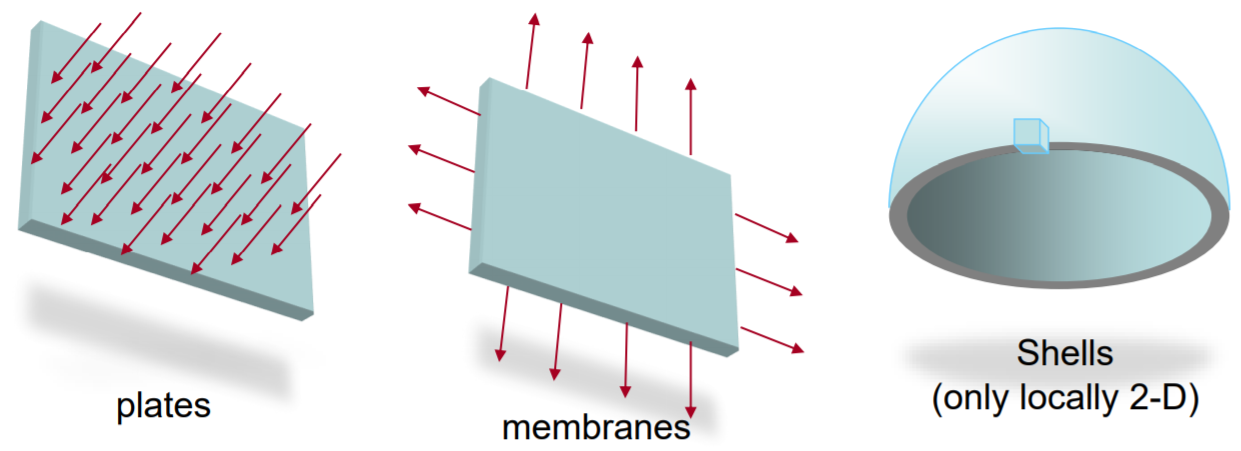
\includegraphics[width = 0.8 \textwidth]{../img/bidimensionalstructures.PNG}
\end{figure}
For shells to be considered bi-dimensional, they need to be looked at very closely where they can resemble a plate. The difference between plates and membranes is the bending rigidity; force is required to bend plates while membranes are really floppy. 
\subsubsection{Mono-dimensional Structures}
If two of the dimensions are negligible compared to the other one, the structure can be studied as mono-dimensional. Some examples are:
\begin{itemize}[noitemsep]
  \item Tie - Prevents two parts of the structure from moving away
  \item Strut - Prevents two parts of the structure from moving forward
  \item Cable - Flexible string that stands only tensile loads
  \item Shaft - Is used for the transmission of torque
  \item Beams - Can carry also transverse loads
\end{itemize}
\begin{figure}[H]
  \centering
  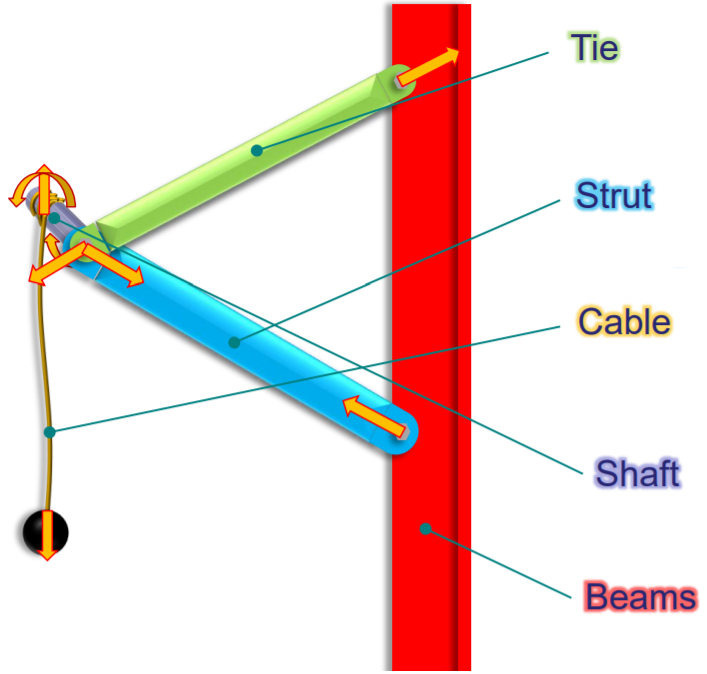
\includegraphics[width = 0.45 \textwidth]{../img/monodimensionalstructures.PNG}
\end{figure}
\subsection{Beams}
The generic mono-dimensional components of structures, able to carry also transverse loads are called \textbf{beams}. Beams are between the most common and important components in structures. In order to study beams as mono-dimensional structures, all mechanical actions have to act on the \textbf{centre of gravity (CG)} of the beam section. If there is a case where a force isn't acting on the CG, it will be converted to act on it, so that the beam can be analysed in a simple manner.
\begin{figure}[H]
  \centering
  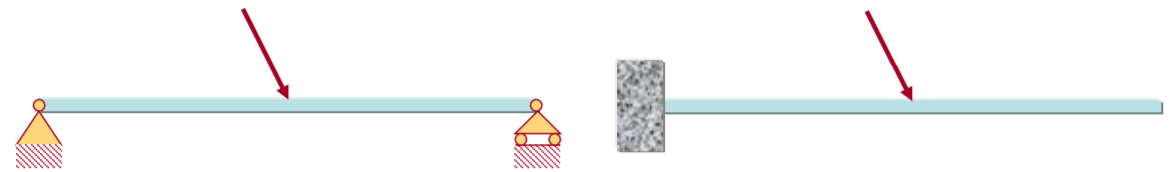
\includegraphics[width = 1 \textwidth]{../img/beamexamples.PNG}
  \caption{On the left: Simply supported beam (rotating support + roller support), On the right: Cantilever beam (with a fixed end)}
\end{figure}
\subsection{Internal Forces}
Each point of the beam is characterised by a specific set of internal forces. We consider a cross section of the beam to investigate these forces.
\begin{figure}[H]
  \centering
  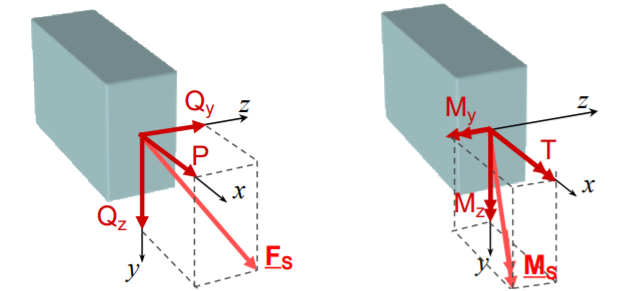
\includegraphics[width = 0.75 \textwidth]{../img/3dinternalforces.PNG}
\end{figure}
\begin{itemize}[noitemsep]
  \item $P$ - Longitudinal force
  \item $Q_y$ - $y$ shear forces
  \item $Q_z$ - $z$ shear forces
  \item $T$ - Torque
  \item $M_y$ - $y$ bending moment
  \item $M_z$ - $z$ bending moment
\end{itemize}
The internal forces at every point of the beam can be characterised with the following expression:
\begin{center}
  $\vec{F} = \left[ \begin{array}{ccccccc} P \\ Q_y \\ Q_z \\ \\ T \\ M_y \\ M_z \end{array}\right]$
\end{center}
In a 2D plane, it simplifies to:
\begin{figure}[H]
  \centering
  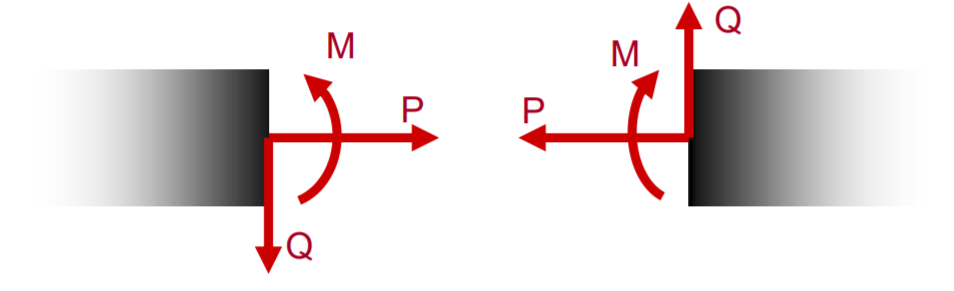
\includegraphics[width = 0.8 \textwidth]{../img/2dinternalforces.PNG}
\end{figure}
\begin{itemize}[noitemsep]
  \item $P$ - Longitudinal force
  \item $Q$ - Shear forces
  \item $M$ - Bending moment
\end{itemize}
\begin{center}
  $\vec{F} = \left[ \begin{array}{ccccccc} P \\ Q \\ M \end{array}\right]$
\end{center}
\subsection{Sign Conventions}
\subsubsection{Longitudional Force}
\begin{figure}[H]
  \centering
  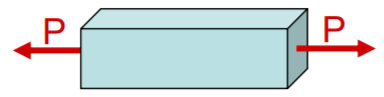
\includegraphics[width = 0.4 \textwidth]{../img/signconventionlongitudionalforce.PNG}
\end{figure}
The direction of pulling is considered to be positive.\\
The direction of compression is considered to be negative.
\subsubsection{Shear Force}
\begin{figure}[H]
  \centering
  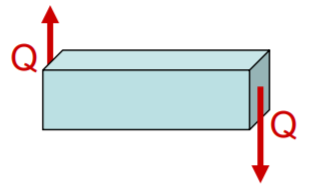
\includegraphics[width = 0.4 \textwidth]{../img/signconventionshearforce.PNG}
\end{figure}
The left side pointing upwards and right side pointing downwards are taken as positive.\\
The left side pointing downwards and right side pointing upwards are taken as negative.
\subsubsection{Bending Moment}
\begin{figure}[H]
  \centering
  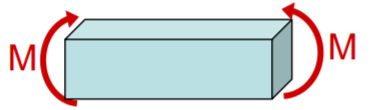
\includegraphics[width = 0.4 \textwidth]{../img/signconventionbendingmoment.PNG}
\end{figure}
If the bending moment is making the beam a upwards concave shape (like U), it is considered to be positive. \\
If the bending moment is making the beam a downwards concave shape, it is considered to be negative.
\subsubsection{Reference System}
\begin{figure}[H]
  \centering
  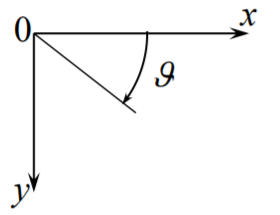
\includegraphics[width = 0.3 \textwidth]{../img/referencesystem.PNG}
\end{figure}
$x$ axis (horizontal direction) to the right is taken as positive. \\
$y$ axis (vertical direction) downwards is taken as positive.

\end{document}